\documentclass[1p]{elsarticle_modified}
%\bibliographystyle{elsarticle-num}

%\usepackage[colorlinks]{hyperref}
%\usepackage{abbrmath_seonhwa} %\Abb, \Ascr, \Acal ,\Abf, \Afrak
\usepackage{amsfonts}
\usepackage{amssymb}
\usepackage{amsmath}
\usepackage{amsthm}
\usepackage{scalefnt}
\usepackage{amsbsy}
\usepackage{kotex}
\usepackage{caption}
\usepackage{subfig}
\usepackage{color}
\usepackage{graphicx}
\usepackage{xcolor} %% white, black, red, green, blue, cyan, magenta, yellow
\usepackage{float}
\usepackage{setspace}
\usepackage{hyperref}

\usepackage{tikz}
\usetikzlibrary{arrows}

\usepackage{multirow}
\usepackage{array} % fixed length table
\usepackage{hhline}

%%%%%%%%%%%%%%%%%%%%%
\makeatletter
\renewcommand*\env@matrix[1][\arraystretch]{%
	\edef\arraystretch{#1}%
	\hskip -\arraycolsep
	\let\@ifnextchar\new@ifnextchar
	\array{*\c@MaxMatrixCols c}}
\makeatother %https://tex.stackexchange.com/questions/14071/how-can-i-increase-the-line-spacing-in-a-matrix
%%%%%%%%%%%%%%%

\usepackage[normalem]{ulem}

\newcommand{\msout}[1]{\ifmmode\text{\sout{\ensuremath{#1}}}\else\sout{#1}\fi}
%SOURCE: \msout is \stkout macro in https://tex.stackexchange.com/questions/20609/strikeout-in-math-mode

\newcommand{\cancel}[1]{
	\ifmmode
	{\color{red}\msout{#1}}
	\else
	{\color{red}\sout{#1}}
	\fi
}

\newcommand{\add}[1]{
	{\color{blue}\uwave{#1}}
}

\newcommand{\replace}[2]{
	\ifmmode
	{\color{red}\msout{#1}}{\color{blue}\uwave{#2}}
	\else
	{\color{red}\sout{#1}}{\color{blue}\uwave{#2}}
	\fi
}

\newcommand{\Sol}{\mathcal{S}} %segment
\newcommand{\D}{D} %diagram
\newcommand{\A}{\mathcal{A}} %arc


%%%%%%%%%%%%%%%%%%%%%%%%%%%%%5 test

\def\sl{\operatorname{\textup{SL}}(2,\Cbb)}
\def\psl{\operatorname{\textup{PSL}}(2,\Cbb)}
\def\quan{\mkern 1mu \triangleright \mkern 1mu}

\theoremstyle{definition}
\newtheorem{thm}{Theorem}[section]
\newtheorem{prop}[thm]{Proposition}
\newtheorem{lem}[thm]{Lemma}
\newtheorem{ques}[thm]{Question}
\newtheorem{cor}[thm]{Corollary}
\newtheorem{defn}[thm]{Definition}
\newtheorem{exam}[thm]{Example}
\newtheorem{rmk}[thm]{Remark}
\newtheorem{alg}[thm]{Algorithm}

\newcommand{\I}{\sqrt{-1}}
\begin{document}

%\begin{frontmatter}
%
%\title{Boundary parabolic representations of knots up to 8 crossings}
%
%%% Group authors per affiliation:
%\author{Yunhi Cho} 
%\address{Department of Mathematics, University of Seoul, Seoul, Korea}
%\ead{yhcho@uos.ac.kr}
%
%
%\author{Seonhwa Kim} %\fnref{s_kim}}
%\address{Center for Geometry and Physics, Institute for Basic Science, Pohang, 37673, Korea}
%\ead{ryeona17@ibs.re.kr}
%
%\author{Hyuk Kim}
%\address{Department of Mathematical Sciences, Seoul National University, Seoul 08826, Korea}
%\ead{hyukkim@snu.ac.kr}
%
%\author{Seokbeom Yoon}
%\address{Department of Mathematical Sciences, Seoul National University, Seoul, 08826,  Korea}
%\ead{sbyoon15@snu.ac.kr}
%
%\begin{abstract}
%We find all boundary parabolic representation of knots up to 8 crossings.
%
%\end{abstract}
%\begin{keyword}
%    \MSC[2010] 57M25 
%\end{keyword}
%
%\end{frontmatter}

%\linenumbers
%\tableofcontents
%
\newcommand\colored[1]{\textcolor{white}{\rule[-0.35ex]{0.8em}{1.4ex}}\kern-0.8em\color{red} #1}%
%\newcommand\colored[1]{\textcolor{white}{ #1}\kern-2.17ex	\textcolor{white}{ #1}\kern-1.81ex	\textcolor{white}{ #1}\kern-2.15ex\color{red}#1	}

{\Large $\underline{12a_{1236}~(K12a_{1236})}$}

\setlength{\tabcolsep}{10pt}
\renewcommand{\arraystretch}{1.6}
\vspace{1cm}\begin{tabular}{m{100pt}>{\centering\arraybackslash}m{274pt}}
\multirow{5}{120pt}{
	\centering
	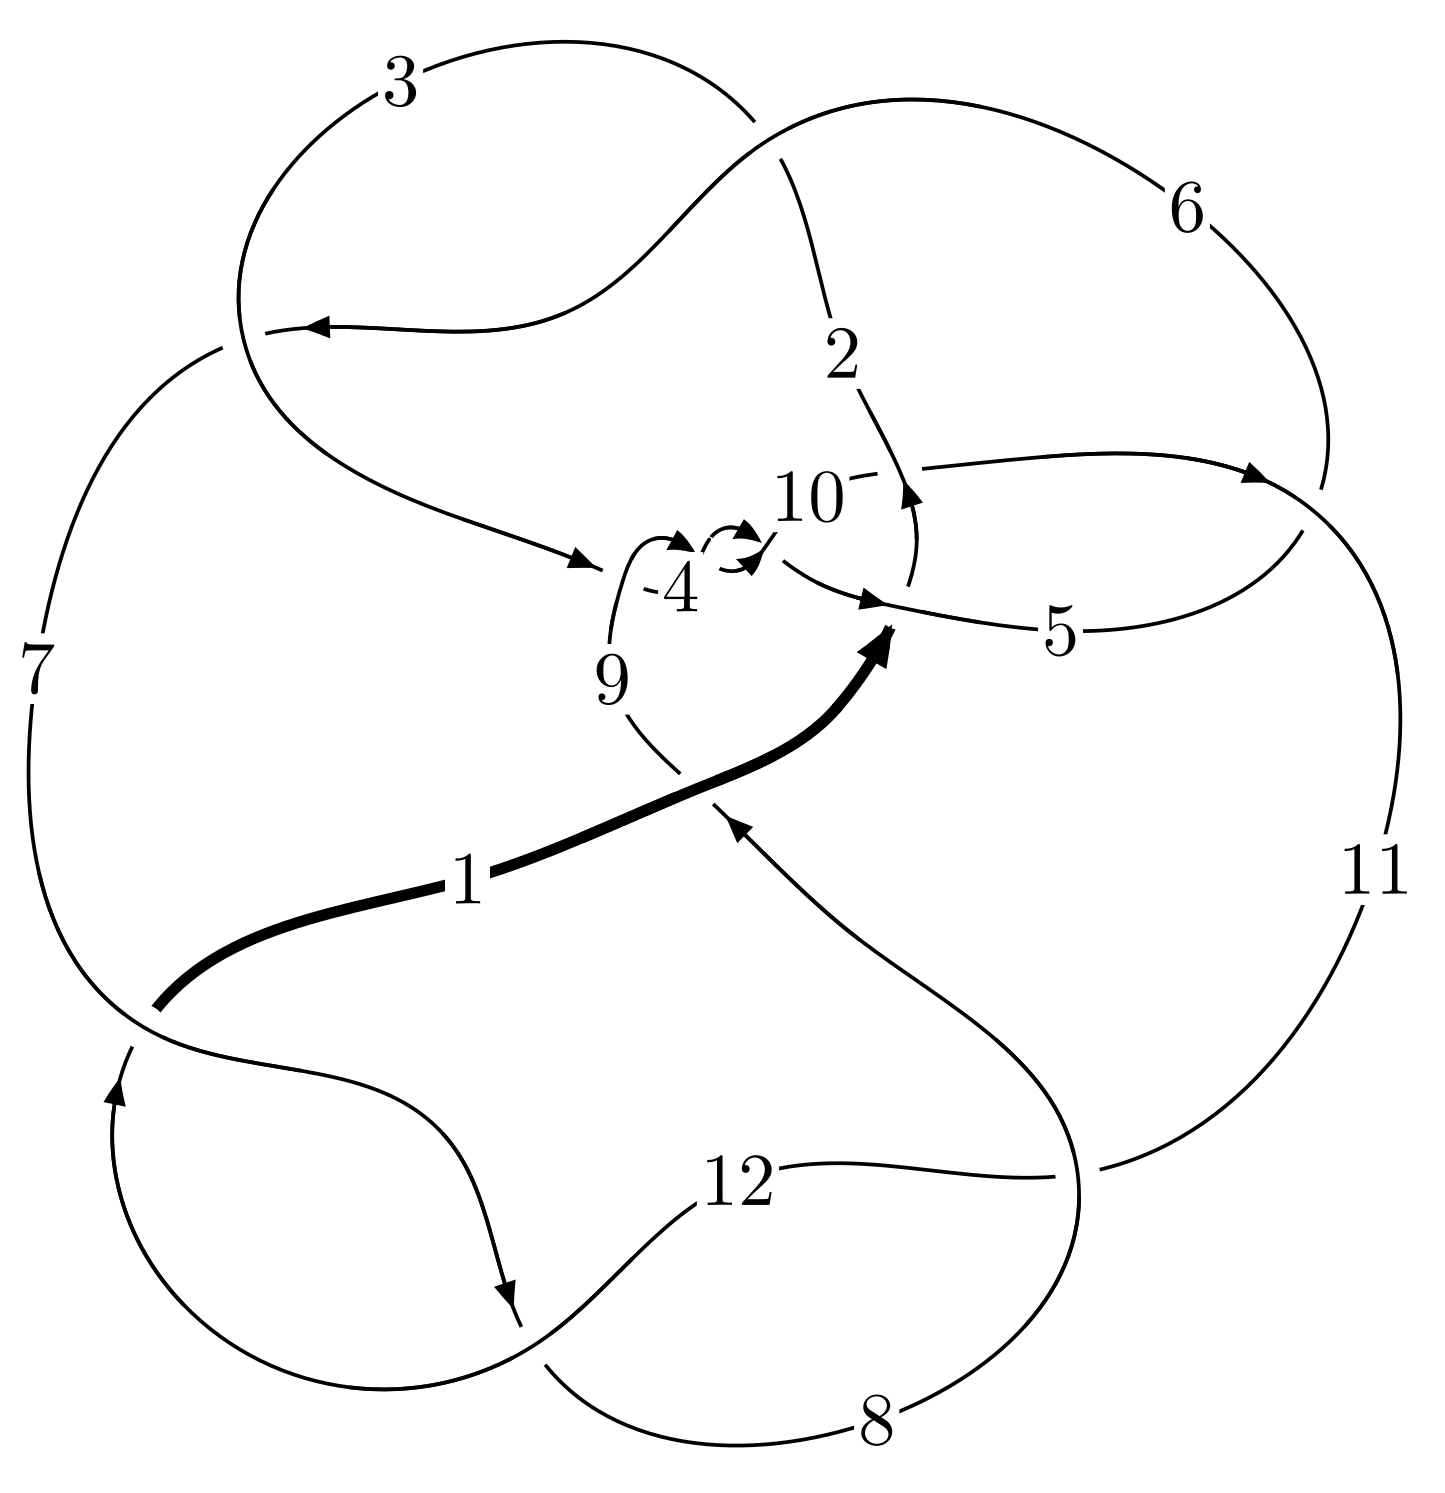
\includegraphics[width=112pt]{../../../GIT/diagram.site/Diagrams/png/2037_12a_1236.png}\\
\ \ \ A knot diagram\footnotemark}&
\allowdisplaybreaks
\textbf{Linearized knot diagam} \\
\cline{2-2}
 &
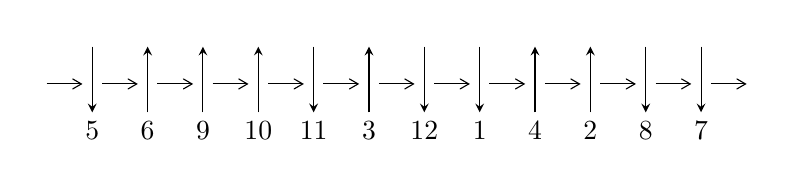
\begin{tikzpicture}[x=20pt, y=17pt]
	% nodes
	\node (C0) at (0, 0) {};
	\node (C1) at (1, 0) {};
	\node (C1U) at (1, +1) {};
	\node (C1D) at (1, -1) {5};

	\node (C2) at (2, 0) {};
	\node (C2U) at (2, +1) {};
	\node (C2D) at (2, -1) {6};

	\node (C3) at (3, 0) {};
	\node (C3U) at (3, +1) {};
	\node (C3D) at (3, -1) {9};

	\node (C4) at (4, 0) {};
	\node (C4U) at (4, +1) {};
	\node (C4D) at (4, -1) {10};

	\node (C5) at (5, 0) {};
	\node (C5U) at (5, +1) {};
	\node (C5D) at (5, -1) {11};

	\node (C6) at (6, 0) {};
	\node (C6U) at (6, +1) {};
	\node (C6D) at (6, -1) {3};

	\node (C7) at (7, 0) {};
	\node (C7U) at (7, +1) {};
	\node (C7D) at (7, -1) {12};

	\node (C8) at (8, 0) {};
	\node (C8U) at (8, +1) {};
	\node (C8D) at (8, -1) {1};

	\node (C9) at (9, 0) {};
	\node (C9U) at (9, +1) {};
	\node (C9D) at (9, -1) {4};

	\node (C10) at (10, 0) {};
	\node (C10U) at (10, +1) {};
	\node (C10D) at (10, -1) {2};

	\node (C11) at (11, 0) {};
	\node (C11U) at (11, +1) {};
	\node (C11D) at (11, -1) {8};

	\node (C12) at (12, 0) {};
	\node (C12U) at (12, +1) {};
	\node (C12D) at (12, -1) {7};
	\node (C13) at (13, 0) {};

	% arrows
	\draw[->,>={angle 60}]
	(C0) edge (C1) (C1) edge (C2) (C2) edge (C3) (C3) edge (C4) (C4) edge (C5) (C5) edge (C6) (C6) edge (C7) (C7) edge (C8) (C8) edge (C9) (C9) edge (C10) (C10) edge (C11) (C11) edge (C12) (C12) edge (C13) ;	\draw[->,>=stealth]
	(C1U) edge (C1D) (C2D) edge (C2U) (C3D) edge (C3U) (C4D) edge (C4U) (C5U) edge (C5D) (C6D) edge (C6U) (C7U) edge (C7D) (C8U) edge (C8D) (C9D) edge (C9U) (C10D) edge (C10U) (C11U) edge (C11D) (C12U) edge (C12D) ;
	\end{tikzpicture} \\
\hhline{~~} \\& 
\textbf{Solving Sequence} \\ \cline{2-2} 
 &
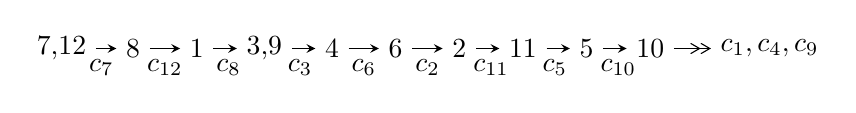
\begin{tikzpicture}[x=23pt, y=7pt]
	% node
	\node (A0) at (-1/8, 0) {7,12};
	\node (A1) at (1, 0) {8};
	\node (A2) at (2, 0) {1};
	\node (A3) at (49/16, 0) {3,9};
	\node (A4) at (33/8, 0) {4};
	\node (A5) at (41/8, 0) {6};
	\node (A6) at (49/8, 0) {2};
	\node (A7) at (57/8, 0) {11};
	\node (A8) at (65/8, 0) {5};
	\node (A9) at (73/8, 0) {10};
	\node (C1) at (1/2, -1) {$c_{7}$};
	\node (C2) at (3/2, -1) {$c_{12}$};
	\node (C3) at (5/2, -1) {$c_{8}$};
	\node (C4) at (29/8, -1) {$c_{3}$};
	\node (C5) at (37/8, -1) {$c_{6}$};
	\node (C6) at (45/8, -1) {$c_{2}$};
	\node (C7) at (53/8, -1) {$c_{11}$};
	\node (C8) at (61/8, -1) {$c_{5}$};
	\node (C9) at (69/8, -1) {$c_{10}$};
	\node (A10) at (11, 0) {$c_{1},c_{4},c_{9}$};

	% edge
	\draw[->,>=stealth]	
	(A0) edge (A1) (A1) edge (A2) (A2) edge (A3) (A3) edge (A4) (A4) edge (A5) (A5) edge (A6) (A6) edge (A7) (A7) edge (A8) (A8) edge (A9) ;
	\draw[->>,>={angle 60}]	
	(A9) edge (A10);
\end{tikzpicture} \\ 

\end{tabular} \\

\footnotetext{
The image of knot diagram is generated by the software ``\textbf{Draw programme}" developed by Andrew Bartholomew(\url{http://www.layer8.co.uk/maths/draw/index.htm\#Running-draw}), where we modified some parts for our purpose(\url{https://github.com/CATsTAILs/LinksPainter}).
}\phantom \\ \newline 
\centering \textbf{Ideals for irreducible components\footnotemark of $X_{\text{par}}$} 
 
\begin{align*}
I^u_{1}&=\langle 
1.42131\times10^{123} u^{103}-8.31432\times10^{122} u^{102}+\cdots+7.88496\times10^{123} b-1.31020\times10^{124},\\
\phantom{I^u_{1}}&\phantom{= \langle  }2.40145\times10^{123} u^{103}+7.06011\times10^{121} u^{102}+\cdots+7.88496\times10^{123} a-3.73579\times10^{124},\\
\phantom{I^u_{1}}&\phantom{= \langle  }u^{104}+48 u^{102}+\cdots-10 u+1\rangle \\
I^u_{2}&=\langle 
- u^{18}- u^{17}+\cdots+b+1,\;-3 u^{19}-3 u^{18}+\cdots+a+2,\;u^{21}+u^{20}+\cdots-2 u-1\rangle \\
\\
\end{align*}
\raggedright * 2 irreducible components of $\dim_{\mathbb{C}}=0$, with total 125 representations.\\
\footnotetext{All coefficients of polynomials are rational numbers. But the coefficients are sometimes approximated in decimal forms when there is not enough margin.}
\newpage
\renewcommand{\arraystretch}{1}
\centering \section*{I. $I^u_{1}= \langle 1.42\times10^{123} u^{103}-8.31\times10^{122} u^{102}+\cdots+7.88\times10^{123} b-1.31\times10^{124},\;2.40\times10^{123} u^{103}+7.06\times10^{121} u^{102}+\cdots+7.88\times10^{123} a-3.74\times10^{124},\;u^{104}+48 u^{102}+\cdots-10 u+1 \rangle$}
\flushleft \textbf{(i) Arc colorings}\\
\begin{tabular}{m{7pt} m{180pt} m{7pt} m{180pt} }
\flushright $a_{7}=$&$\begin{pmatrix}1\\0\end{pmatrix}$ \\
\flushright $a_{12}=$&$\begin{pmatrix}0\\u\end{pmatrix}$ \\
\flushright $a_{8}=$&$\begin{pmatrix}1\\u^2\end{pmatrix}$ \\
\flushright $a_{1}=$&$\begin{pmatrix}- u\\u\end{pmatrix}$ \\
\flushright $a_{3}=$&$\begin{pmatrix}-0.304561 u^{103}-0.00895389 u^{102}+\cdots-5.28918 u+4.73786\\-0.180256 u^{103}+0.105445 u^{102}+\cdots-0.205229 u+1.66165\end{pmatrix}$ \\
\flushright $a_{9}=$&$\begin{pmatrix}- u^4- u^2+1\\u^4+2 u^2\end{pmatrix}$ \\
\flushright $a_{4}=$&$\begin{pmatrix}-0.503681 u^{103}-0.0491159 u^{102}+\cdots-5.68605 u+6.33520\\-0.141227 u^{103}+0.133202 u^{102}+\cdots-0.273063 u+1.70134\end{pmatrix}$ \\
\flushright $a_{6}=$&$\begin{pmatrix}-0.754616 u^{103}-0.358618 u^{102}+\cdots-1.06064 u+8.36278\\-0.163006 u^{103}+0.0997843 u^{102}+\cdots-2.03954 u+3.07367\end{pmatrix}$ \\
\flushright $a_{2}=$&$\begin{pmatrix}1.30230 u^{103}+0.259004 u^{102}+\cdots-0.111082 u-10.0921\\0.441501 u^{103}-0.0875902 u^{102}+\cdots+3.77303 u-3.80556\end{pmatrix}$ \\
\flushright $a_{11}=$&$\begin{pmatrix}u\\u^3+u\end{pmatrix}$ \\
\flushright $a_{5}=$&$\begin{pmatrix}-0.873306 u^{103}-0.247297 u^{102}+\cdots-1.79375 u+8.39105\\-0.0628994 u^{103}+0.0596347 u^{102}+\cdots-1.54074 u+2.99062\end{pmatrix}$ \\
\flushright $a_{10}=$&$\begin{pmatrix}0.688002 u^{103}-0.203148 u^{102}+\cdots+8.09484 u-9.31886\\0.212943 u^{103}+0.326702 u^{102}+\cdots-0.785101 u-2.66788\end{pmatrix}$\\&\end{tabular}
\flushleft \textbf{(ii) Obstruction class $= -1$}\\~\\
\flushleft \textbf{(iii) Cusp Shapes $= -3.09066 u^{103}-0.418692 u^{102}+\cdots-10.7066 u+25.3820$}\\~\\
\newpage\renewcommand{\arraystretch}{1}
\flushleft \textbf{(iv) u-Polynomials at the component}\newline \\
\begin{tabular}{m{50pt}|m{274pt}}
Crossings & \hspace{64pt}u-Polynomials at each crossing \\
\hline $$\begin{aligned}c_{1}\end{aligned}$$&$\begin{aligned}
&u^{104}+7 u^{103}+\cdots-906 u+1909
\end{aligned}$\\
\hline $$\begin{aligned}c_{2},c_{6}\end{aligned}$$&$\begin{aligned}
&u^{104}+2 u^{103}+\cdots+63 u+73
\end{aligned}$\\
\hline $$\begin{aligned}c_{3},c_{4},c_{9}\end{aligned}$$&$\begin{aligned}
&u^{104}- u^{103}+\cdots-42 u-1
\end{aligned}$\\
\hline $$\begin{aligned}c_{5}\end{aligned}$$&$\begin{aligned}
&u^{104}+u^{103}+\cdots-106 u+1
\end{aligned}$\\
\hline $$\begin{aligned}c_{7},c_{11},c_{12}\end{aligned}$$&$\begin{aligned}
&u^{104}+48 u^{102}+\cdots+10 u+1
\end{aligned}$\\
\hline $$\begin{aligned}c_{8}\end{aligned}$$&$\begin{aligned}
&u^{104}- u^{101}+\cdots+7744 u+457
\end{aligned}$\\
\hline $$\begin{aligned}c_{10}\end{aligned}$$&$\begin{aligned}
&u^{104}-5 u^{103}+\cdots-39735 u+17047
\end{aligned}$\\
\hline
\end{tabular}\\~\\
\newpage\renewcommand{\arraystretch}{1}
\flushleft \textbf{(v) Riley Polynomials at the component}\newline \\
\begin{tabular}{m{50pt}|m{274pt}}
Crossings & \hspace{64pt}Riley Polynomials at each crossing \\
\hline $$\begin{aligned}c_{1}\end{aligned}$$&$\begin{aligned}
&y^{104}+23 y^{103}+\cdots+88027842 y+3644281
\end{aligned}$\\
\hline $$\begin{aligned}c_{2},c_{6}\end{aligned}$$&$\begin{aligned}
&y^{104}-82 y^{103}+\cdots+131957 y+5329
\end{aligned}$\\
\hline $$\begin{aligned}c_{3},c_{4},c_{9}\end{aligned}$$&$\begin{aligned}
&y^{104}-109 y^{103}+\cdots-1178 y+1
\end{aligned}$\\
\hline $$\begin{aligned}c_{5}\end{aligned}$$&$\begin{aligned}
&y^{104}+15 y^{103}+\cdots-10638 y+1
\end{aligned}$\\
\hline $$\begin{aligned}c_{7},c_{11},c_{12}\end{aligned}$$&$\begin{aligned}
&y^{104}+96 y^{103}+\cdots-72 y+1
\end{aligned}$\\
\hline $$\begin{aligned}c_{8}\end{aligned}$$&$\begin{aligned}
&y^{104}+106 y^{102}+\cdots-16677012 y+208849
\end{aligned}$\\
\hline $$\begin{aligned}c_{10}\end{aligned}$$&$\begin{aligned}
&y^{104}-41 y^{103}+\cdots-14746825375 y+290600209
\end{aligned}$\\
\hline
\end{tabular}\\~\\
\newpage\flushleft \textbf{(vi) Complex Volumes and Cusp Shapes}
$$\begin{array}{c|c|c}  
\text{Solutions to }I^u_{1}& \I (\text{vol} + \sqrt{-1}CS) & \text{Cusp shape}\\
 \hline 
\begin{aligned}
u &= \phantom{-}0.620118 + 0.789865 I \\
a &= \phantom{-}0.521286 + 0.592077 I \\
b &= -1.35459 - 0.45056 I\end{aligned}
 & \phantom{-}9.56661 + 8.03524 I & \phantom{-0.000000 } 0 \\ \hline\begin{aligned}
u &= \phantom{-}0.620118 - 0.789865 I \\
a &= \phantom{-}0.521286 - 0.592077 I \\
b &= -1.35459 + 0.45056 I\end{aligned}
 & \phantom{-}9.56661 - 8.03524 I & \phantom{-0.000000 } 0 \\ \hline\begin{aligned}
u &= -0.105335 + 1.030070 I \\
a &= \phantom{-}1.51620 - 0.42594 I \\
b &= -0.385243 + 0.617360 I\end{aligned}
 & \phantom{-}5.10809 + 3.63975 I & \phantom{-0.000000 } 0 \\ \hline\begin{aligned}
u &= -0.105335 - 1.030070 I \\
a &= \phantom{-}1.51620 + 0.42594 I \\
b &= -0.385243 - 0.617360 I\end{aligned}
 & \phantom{-}5.10809 - 3.63975 I & \phantom{-0.000000 } 0 \\ \hline\begin{aligned}
u &= -1.03778\phantom{ +0.000000I} \\
a &= -0.0269272\phantom{ +0.000000I} \\
b &= -1.07237\phantom{ +0.000000I}\end{aligned}
 & \phantom{-}3.29245\phantom{ +0.000000I} & \phantom{-0.000000 } 0 \\ \hline\begin{aligned}
u &= -0.746382 + 0.602859 I \\
a &= \phantom{-}0.998714 - 0.840032 I \\
b &= -0.855899 - 0.402358 I\end{aligned}
 & \phantom{-}3.94155 + 4.30366 I & \phantom{-0.000000 } 0 \\ \hline\begin{aligned}
u &= -0.746382 - 0.602859 I \\
a &= \phantom{-}0.998714 + 0.840032 I \\
b &= -0.855899 + 0.402358 I\end{aligned}
 & \phantom{-}3.94155 - 4.30366 I & \phantom{-0.000000 } 0 \\ \hline\begin{aligned}
u &= \phantom{-}0.829680 + 0.352824 I \\
a &= \phantom{-}0.565617 + 1.157080 I \\
b &= -1.41176 + 0.56699 I\end{aligned}
 & \phantom{-}8.2061 - 13.0082 I & \phantom{-0.000000 } 0 \\ \hline\begin{aligned}
u &= \phantom{-}0.829680 - 0.352824 I \\
a &= \phantom{-}0.565617 - 1.157080 I \\
b &= -1.41176 - 0.56699 I\end{aligned}
 & \phantom{-}8.2061 + 13.0082 I & \phantom{-0.000000 } 0 \\ \hline\begin{aligned}
u &= -0.154977 + 1.099720 I \\
a &= -0.834959 - 0.027034 I \\
b &= \phantom{-}0.308767 + 0.799992 I\end{aligned}
 & \phantom{-}0.087281 - 0.510738 I & \phantom{-0.000000 } 0\\
 \hline 
 \end{array}$$\newpage$$\begin{array}{c|c|c}  
\text{Solutions to }I^u_{1}& \I (\text{vol} + \sqrt{-1}CS) & \text{Cusp shape}\\
 \hline 
\begin{aligned}
u &= -0.154977 - 1.099720 I \\
a &= -0.834959 + 0.027034 I \\
b &= \phantom{-}0.308767 - 0.799992 I\end{aligned}
 & \phantom{-}0.087281 + 0.510738 I & \phantom{-0.000000 } 0 \\ \hline\begin{aligned}
u &= \phantom{-}0.191981 + 0.865189 I \\
a &= -0.082965 - 0.736955 I \\
b &= \phantom{-}1.340770 + 0.359873 I\end{aligned}
 & \phantom{-}9.58062 - 0.35742 I & \phantom{-0.000000 } 0 \\ \hline\begin{aligned}
u &= \phantom{-}0.191981 - 0.865189 I \\
a &= -0.082965 + 0.736955 I \\
b &= \phantom{-}1.340770 - 0.359873 I\end{aligned}
 & \phantom{-}9.58062 + 0.35742 I & \phantom{-0.000000 } 0 \\ \hline\begin{aligned}
u &= \phantom{-}0.857934\phantom{ +0.000000I} \\
a &= -0.114455\phantom{ +0.000000I} \\
b &= \phantom{-}0.723712\phantom{ +0.000000I}\end{aligned}
 & -1.60767\phantom{ +0.000000I} & -15.4730\phantom{ +0.000000I} \\ \hline\begin{aligned}
u &= \phantom{-}0.367285 + 1.109370 I \\
a &= -0.960640 - 0.313248 I \\
b &= \phantom{-}0.861427 - 0.337448 I\end{aligned}
 & \phantom{-}1.80378 - 4.43282 I & \phantom{-0.000000 } 0 \\ \hline\begin{aligned}
u &= \phantom{-}0.367285 - 1.109370 I \\
a &= -0.960640 + 0.313248 I \\
b &= \phantom{-}0.861427 + 0.337448 I\end{aligned}
 & \phantom{-}1.80378 + 4.43282 I & \phantom{-0.000000 } 0 \\ \hline\begin{aligned}
u &= -0.408974 + 0.720777 I \\
a &= -1.010150 + 0.592828 I \\
b &= \phantom{-}1.171700 - 0.398512 I\end{aligned}
 & \phantom{-}2.81966 - 4.74793 I & \phantom{-}3.70519 + 4.52321 I \\ \hline\begin{aligned}
u &= -0.408974 - 0.720777 I \\
a &= -1.010150 - 0.592828 I \\
b &= \phantom{-}1.171700 + 0.398512 I\end{aligned}
 & \phantom{-}2.81966 + 4.74793 I & \phantom{-}3.70519 - 4.52321 I \\ \hline\begin{aligned}
u &= \phantom{-}0.043813 + 1.200940 I \\
a &= \phantom{-}1.50087 - 0.34043 I \\
b &= -1.093100 - 0.538555 I\end{aligned}
 & \phantom{-}3.93615 + 1.11713 I & \phantom{-0.000000 } 0 \\ \hline\begin{aligned}
u &= \phantom{-}0.043813 - 1.200940 I \\
a &= \phantom{-}1.50087 + 0.34043 I \\
b &= -1.093100 + 0.538555 I\end{aligned}
 & \phantom{-}3.93615 - 1.11713 I & \phantom{-0.000000 } 0\\
 \hline 
 \end{array}$$\newpage$$\begin{array}{c|c|c}  
\text{Solutions to }I^u_{1}& \I (\text{vol} + \sqrt{-1}CS) & \text{Cusp shape}\\
 \hline 
\begin{aligned}
u &= \phantom{-}0.695428 + 0.387530 I \\
a &= -0.813314 - 0.738577 I \\
b &= \phantom{-}0.910790 - 0.218196 I\end{aligned}
 & -0.45127 - 2.08949 I & -5.67320 + 7.54122 I \\ \hline\begin{aligned}
u &= \phantom{-}0.695428 - 0.387530 I \\
a &= -0.813314 + 0.738577 I \\
b &= \phantom{-}0.910790 + 0.218196 I\end{aligned}
 & -0.45127 + 2.08949 I & -5.67320 - 7.54122 I \\ \hline\begin{aligned}
u &= -0.735924 + 0.296284 I \\
a &= -0.80397 + 1.25813 I \\
b &= \phantom{-}1.303710 + 0.471076 I\end{aligned}
 & \phantom{-}1.35265 + 8.84857 I & \phantom{-}1.14263 - 8.81074 I \\ \hline\begin{aligned}
u &= -0.735924 - 0.296284 I \\
a &= -0.80397 - 1.25813 I \\
b &= \phantom{-}1.303710 - 0.471076 I\end{aligned}
 & \phantom{-}1.35265 - 8.84857 I & \phantom{-}1.14263 + 8.81074 I \\ \hline\begin{aligned}
u &= -0.705894 + 0.351680 I \\
a &= \phantom{-}0.188275 + 0.274678 I \\
b &= -0.551335 + 0.540399 I\end{aligned}
 & \phantom{-}3.17492 + 0.39098 I & \phantom{-}0.93290 - 2.00106 I \\ \hline\begin{aligned}
u &= -0.705894 - 0.351680 I \\
a &= \phantom{-}0.188275 - 0.274678 I \\
b &= -0.551335 - 0.540399 I\end{aligned}
 & \phantom{-}3.17492 - 0.39098 I & \phantom{-}0.93290 + 2.00106 I \\ \hline\begin{aligned}
u &= -0.722198 + 0.274964 I \\
a &= \phantom{-}0.19760 + 1.63490 I \\
b &= \phantom{-}1.194830 + 0.126529 I\end{aligned}
 & \phantom{-}8.05202 + 4.22912 I & \phantom{-}6.55587 - 4.57124 I \\ \hline\begin{aligned}
u &= -0.722198 - 0.274964 I \\
a &= \phantom{-}0.19760 - 1.63490 I \\
b &= \phantom{-}1.194830 - 0.126529 I\end{aligned}
 & \phantom{-}8.05202 - 4.22912 I & \phantom{-}6.55587 + 4.57124 I \\ \hline\begin{aligned}
u &= -0.771734\phantom{ +0.000000I} \\
a &= \phantom{-}0.759937\phantom{ +0.000000I} \\
b &= -0.790368\phantom{ +0.000000I}\end{aligned}
 & \phantom{-}2.40158\phantom{ +0.000000I} & \phantom{-}5.63180\phantom{ +0.000000I} \\ \hline\begin{aligned}
u &= -0.246560 + 0.725443 I \\
a &= -0.446882 - 0.239528 I \\
b &= \phantom{-}1.329300 + 0.122327 I\end{aligned}
 & \phantom{-}9.68887 - 0.42429 I & \phantom{-}9.29933 - 1.12741 I\\
 \hline 
 \end{array}$$\newpage$$\begin{array}{c|c|c}  
\text{Solutions to }I^u_{1}& \I (\text{vol} + \sqrt{-1}CS) & \text{Cusp shape}\\
 \hline 
\begin{aligned}
u &= -0.246560 - 0.725443 I \\
a &= -0.446882 + 0.239528 I \\
b &= \phantom{-}1.329300 - 0.122327 I\end{aligned}
 & \phantom{-}9.68887 + 0.42429 I & \phantom{-}9.29933 + 1.12741 I \\ \hline\begin{aligned}
u &= \phantom{-}0.716700 + 0.247198 I \\
a &= \phantom{-}0.11399 - 1.50069 I \\
b &= \phantom{-}1.44713 - 0.71686 I\end{aligned}
 & \phantom{-}7.66319 - 3.32471 I & \phantom{-}7.08153 + 4.25402 I \\ \hline\begin{aligned}
u &= \phantom{-}0.716700 - 0.247198 I \\
a &= \phantom{-}0.11399 + 1.50069 I \\
b &= \phantom{-}1.44713 + 0.71686 I\end{aligned}
 & \phantom{-}7.66319 + 3.32471 I & \phantom{-}7.08153 - 4.25402 I \\ \hline\begin{aligned}
u &= \phantom{-}0.243166 + 1.243460 I \\
a &= \phantom{-}0.202575 + 0.189137 I \\
b &= -0.284679 + 0.591002 I\end{aligned}
 & \phantom{-}1.66136 - 3.20269 I & \phantom{-0.000000 } 0 \\ \hline\begin{aligned}
u &= \phantom{-}0.243166 - 1.243460 I \\
a &= \phantom{-}0.202575 - 0.189137 I \\
b &= -0.284679 - 0.591002 I\end{aligned}
 & \phantom{-}1.66136 + 3.20269 I & \phantom{-0.000000 } 0 \\ \hline\begin{aligned}
u &= \phantom{-}0.665439 + 0.274419 I \\
a &= -0.332478 - 0.928461 I \\
b &= \phantom{-}0.011124 - 1.285510 I\end{aligned}
 & \phantom{-}3.67182 - 6.63904 I & \phantom{-}1.49843 + 7.92289 I \\ \hline\begin{aligned}
u &= \phantom{-}0.665439 - 0.274419 I \\
a &= -0.332478 + 0.928461 I \\
b &= \phantom{-}0.011124 + 1.285510 I\end{aligned}
 & \phantom{-}3.67182 + 6.63904 I & \phantom{-}1.49843 - 7.92289 I \\ \hline\begin{aligned}
u &= -0.080589 + 1.296550 I \\
a &= -0.078900 - 0.672379 I \\
b &= -0.614973 + 0.771669 I\end{aligned}
 & \phantom{-}4.80034 - 1.11455 I & \phantom{-0.000000 } 0 \\ \hline\begin{aligned}
u &= -0.080589 - 1.296550 I \\
a &= -0.078900 + 0.672379 I \\
b &= -0.614973 - 0.771669 I\end{aligned}
 & \phantom{-}4.80034 + 1.11455 I & \phantom{-0.000000 } 0 \\ \hline\begin{aligned}
u &= \phantom{-}0.698700 + 0.022216 I \\
a &= -0.527324 - 0.318258 I \\
b &= -0.041523 - 0.373581 I\end{aligned}
 & -2.08518 - 0.19609 I & -5.25700 - 1.07973 I\\
 \hline 
 \end{array}$$\newpage$$\begin{array}{c|c|c}  
\text{Solutions to }I^u_{1}& \I (\text{vol} + \sqrt{-1}CS) & \text{Cusp shape}\\
 \hline 
\begin{aligned}
u &= \phantom{-}0.698700 - 0.022216 I \\
a &= -0.527324 + 0.318258 I \\
b &= -0.041523 + 0.373581 I\end{aligned}
 & -2.08518 + 0.19609 I & -5.25700 + 1.07973 I \\ \hline\begin{aligned}
u &= -0.682573 + 0.149623 I \\
a &= \phantom{-}0.368074 - 0.719379 I \\
b &= \phantom{-}0.042810 - 0.956572 I\end{aligned}
 & -2.61203 + 3.75303 I & -4.16251 - 7.39345 I \\ \hline\begin{aligned}
u &= -0.682573 - 0.149623 I \\
a &= \phantom{-}0.368074 + 0.719379 I \\
b &= \phantom{-}0.042810 + 0.956572 I\end{aligned}
 & -2.61203 - 3.75303 I & -4.16251 + 7.39345 I \\ \hline\begin{aligned}
u &= \phantom{-}0.071296 + 1.310970 I \\
a &= -0.071099 - 0.804873 I \\
b &= -0.427448 + 0.028098 I\end{aligned}
 & \phantom{-}4.95252 - 1.57160 I & \phantom{-0.000000 } 0 \\ \hline\begin{aligned}
u &= \phantom{-}0.071296 - 1.310970 I \\
a &= -0.071099 + 0.804873 I \\
b &= -0.427448 - 0.028098 I\end{aligned}
 & \phantom{-}4.95252 + 1.57160 I & \phantom{-0.000000 } 0 \\ \hline\begin{aligned}
u &= \phantom{-}0.303223 + 1.286920 I \\
a &= -0.587063 + 0.148446 I \\
b &= \phantom{-}0.088712 - 0.174045 I\end{aligned}
 & \phantom{-}1.98304 - 3.83783 I & \phantom{-0.000000 } 0 \\ \hline\begin{aligned}
u &= \phantom{-}0.303223 - 1.286920 I \\
a &= -0.587063 - 0.148446 I \\
b &= \phantom{-}0.088712 + 0.174045 I\end{aligned}
 & \phantom{-}1.98304 + 3.83783 I & \phantom{-0.000000 } 0 \\ \hline\begin{aligned}
u &= -0.573315 + 1.219970 I \\
a &= \phantom{-}0.718100 - 0.491528 I \\
b &= -1.111370 - 0.127817 I\end{aligned}
 & \phantom{-}7.02373 + 5.61735 I & \phantom{-0.000000 } 0 \\ \hline\begin{aligned}
u &= -0.573315 - 1.219970 I \\
a &= \phantom{-}0.718100 + 0.491528 I \\
b &= -1.111370 + 0.127817 I\end{aligned}
 & \phantom{-}7.02373 - 5.61735 I & \phantom{-0.000000 } 0 \\ \hline\begin{aligned}
u &= -0.273407 + 1.343450 I \\
a &= \phantom{-}0.849372 + 0.471844 I \\
b &= -0.087968 - 1.038730 I\end{aligned}
 & \phantom{-}2.09247 + 7.22215 I & \phantom{-0.000000 } 0\\
 \hline 
 \end{array}$$\newpage$$\begin{array}{c|c|c}  
\text{Solutions to }I^u_{1}& \I (\text{vol} + \sqrt{-1}CS) & \text{Cusp shape}\\
 \hline 
\begin{aligned}
u &= -0.273407 - 1.343450 I \\
a &= \phantom{-}0.849372 - 0.471844 I \\
b &= -0.087968 + 1.038730 I\end{aligned}
 & \phantom{-}2.09247 - 7.22215 I & \phantom{-0.000000 } 0 \\ \hline\begin{aligned}
u &= \phantom{-}0.569902 + 0.259753 I \\
a &= \phantom{-}1.47098 + 1.16159 I \\
b &= -1.250830 + 0.290569 I\end{aligned}
 & \phantom{-}1.59615 - 3.09335 I & \phantom{-}3.07050 + 7.96279 I \\ \hline\begin{aligned}
u &= \phantom{-}0.569902 - 0.259753 I \\
a &= \phantom{-}1.47098 - 1.16159 I \\
b &= -1.250830 - 0.290569 I\end{aligned}
 & \phantom{-}1.59615 + 3.09335 I & \phantom{-}3.07050 - 7.96279 I \\ \hline\begin{aligned}
u &= \phantom{-}0.064615 + 1.389110 I \\
a &= -2.69390 - 0.27554 I \\
b &= \phantom{-}1.130990 - 0.439667 I\end{aligned}
 & \phantom{-}9.11640 - 3.79729 I & \phantom{-0.000000 } 0 \\ \hline\begin{aligned}
u &= \phantom{-}0.064615 - 1.389110 I \\
a &= -2.69390 + 0.27554 I \\
b &= \phantom{-}1.130990 + 0.439667 I\end{aligned}
 & \phantom{-}9.11640 + 3.79729 I & \phantom{-0.000000 } 0 \\ \hline\begin{aligned}
u &= -0.217418 + 1.379800 I \\
a &= \phantom{-}1.97103 - 0.92033 I \\
b &= -1.399880 + 0.080986 I\end{aligned}
 & \phantom{-}6.95103 + 2.47096 I & \phantom{-0.000000 } 0 \\ \hline\begin{aligned}
u &= -0.217418 - 1.379800 I \\
a &= \phantom{-}1.97103 + 0.92033 I \\
b &= -1.399880 - 0.080986 I\end{aligned}
 & \phantom{-}6.95103 - 2.47096 I & \phantom{-0.000000 } 0 \\ \hline\begin{aligned}
u &= \phantom{-}0.131274 + 1.392020 I \\
a &= -2.35695 - 1.10644 I \\
b &= \phantom{-}2.03046 + 0.39544 I\end{aligned}
 & \phantom{-}15.1827 - 1.2684 I & \phantom{-0.000000 } 0 \\ \hline\begin{aligned}
u &= \phantom{-}0.131274 - 1.392020 I \\
a &= -2.35695 + 1.10644 I \\
b &= \phantom{-}2.03046 - 0.39544 I\end{aligned}
 & \phantom{-}15.1827 + 1.2684 I & \phantom{-0.000000 } 0 \\ \hline\begin{aligned}
u &= -0.212116 + 1.389820 I \\
a &= \phantom{-}2.20201 - 0.82635 I \\
b &= -1.35433 - 0.67085 I\end{aligned}
 & \phantom{-}6.99266 + 5.38612 I & \phantom{-0.000000 } 0\\
 \hline 
 \end{array}$$\newpage$$\begin{array}{c|c|c}  
\text{Solutions to }I^u_{1}& \I (\text{vol} + \sqrt{-1}CS) & \text{Cusp shape}\\
 \hline 
\begin{aligned}
u &= -0.212116 - 1.389820 I \\
a &= \phantom{-}2.20201 + 0.82635 I \\
b &= -1.35433 + 0.67085 I\end{aligned}
 & \phantom{-}6.99266 - 5.38612 I & \phantom{-0.000000 } 0 \\ \hline\begin{aligned}
u &= \phantom{-}0.20338 + 1.40110 I \\
a &= \phantom{-}2.12985 + 1.61341 I \\
b &= -1.160280 + 0.081319 I\end{aligned}
 & \phantom{-}7.27022 - 2.24226 I & \phantom{-0.000000 } 0 \\ \hline\begin{aligned}
u &= \phantom{-}0.20338 - 1.40110 I \\
a &= \phantom{-}2.12985 - 1.61341 I \\
b &= -1.160280 - 0.081319 I\end{aligned}
 & \phantom{-}7.27022 + 2.24226 I & \phantom{-0.000000 } 0 \\ \hline\begin{aligned}
u &= \phantom{-}0.16109 + 1.40977 I \\
a &= \phantom{-}0.120261 - 0.660060 I \\
b &= \phantom{-}0.673479 + 1.217030 I\end{aligned}
 & \phantom{-}10.51900 + 1.46499 I & \phantom{-0.000000 } 0 \\ \hline\begin{aligned}
u &= \phantom{-}0.16109 - 1.40977 I \\
a &= \phantom{-}0.120261 + 0.660060 I \\
b &= \phantom{-}0.673479 - 1.217030 I\end{aligned}
 & \phantom{-}10.51900 - 1.46499 I & \phantom{-0.000000 } 0 \\ \hline\begin{aligned}
u &= \phantom{-}0.22769 + 1.40184 I \\
a &= \phantom{-}2.73223 + 0.77856 I \\
b &= -1.384850 + 0.232626 I\end{aligned}
 & \phantom{-}6.91603 - 6.05149 I & \phantom{-0.000000 } 0 \\ \hline\begin{aligned}
u &= \phantom{-}0.22769 - 1.40184 I \\
a &= \phantom{-}2.73223 - 0.77856 I \\
b &= -1.384850 - 0.232626 I\end{aligned}
 & \phantom{-}6.91603 + 6.05149 I & \phantom{-0.000000 } 0 \\ \hline\begin{aligned}
u &= -0.12690 + 1.41514 I \\
a &= -2.49800 + 0.06442 I \\
b &= \phantom{-}1.57856 - 0.11426 I\end{aligned}
 & \phantom{-}15.7422 + 0.8659 I & \phantom{-0.000000 } 0 \\ \hline\begin{aligned}
u &= -0.12690 - 1.41514 I \\
a &= -2.49800 - 0.06442 I \\
b &= \phantom{-}1.57856 + 0.11426 I\end{aligned}
 & \phantom{-}15.7422 - 0.8659 I & \phantom{-0.000000 } 0 \\ \hline\begin{aligned}
u &= -0.14866 + 1.41986 I \\
a &= -0.023453 - 0.800359 I \\
b &= \phantom{-}0.363945 - 0.398775 I\end{aligned}
 & \phantom{-}10.64610 + 5.13547 I & \phantom{-0.000000 } 0\\
 \hline 
 \end{array}$$\newpage$$\begin{array}{c|c|c}  
\text{Solutions to }I^u_{1}& \I (\text{vol} + \sqrt{-1}CS) & \text{Cusp shape}\\
 \hline 
\begin{aligned}
u &= -0.14866 - 1.41986 I \\
a &= -0.023453 + 0.800359 I \\
b &= \phantom{-}0.363945 + 0.398775 I\end{aligned}
 & \phantom{-}10.64610 - 5.13547 I & \phantom{-0.000000 } 0 \\ \hline\begin{aligned}
u &= -0.516954 + 0.237865 I \\
a &= \phantom{-}0.35640 - 1.91087 I \\
b &= -1.132780 - 0.585934 I\end{aligned}
 & \phantom{-}1.79267 + 2.64792 I & \phantom{-}4.98022 - 10.27183 I \\ \hline\begin{aligned}
u &= -0.516954 - 0.237865 I \\
a &= \phantom{-}0.35640 + 1.91087 I \\
b &= -1.132780 + 0.585934 I\end{aligned}
 & \phantom{-}1.79267 - 2.64792 I & \phantom{-}4.98022 + 10.27183 I \\ \hline\begin{aligned}
u &= \phantom{-}0.28290 + 1.40368 I \\
a &= -1.99965 - 0.89852 I \\
b &= \phantom{-}1.55247 - 0.88840 I\end{aligned}
 & \phantom{-}12.9310 - 6.9544 I & \phantom{-0.000000 } 0 \\ \hline\begin{aligned}
u &= \phantom{-}0.28290 - 1.40368 I \\
a &= -1.99965 + 0.89852 I \\
b &= \phantom{-}1.55247 + 0.88840 I\end{aligned}
 & \phantom{-}12.9310 + 6.9544 I & \phantom{-0.000000 } 0 \\ \hline\begin{aligned}
u &= -0.09297 + 1.42903 I \\
a &= -2.51248 + 0.76287 I \\
b &= \phantom{-}1.187870 - 0.152148 I\end{aligned}
 & \phantom{-}9.54976 - 3.46045 I & \phantom{-0.000000 } 0 \\ \hline\begin{aligned}
u &= -0.09297 - 1.42903 I \\
a &= -2.51248 - 0.76287 I \\
b &= \phantom{-}1.187870 + 0.152148 I\end{aligned}
 & \phantom{-}9.54976 + 3.46045 I & \phantom{-0.000000 } 0 \\ \hline\begin{aligned}
u &= \phantom{-}0.26025 + 1.41053 I \\
a &= -0.868443 + 0.711871 I \\
b &= \phantom{-}0.07049 - 1.49738 I\end{aligned}
 & \phantom{-}9.05860 - 10.01860 I & \phantom{-0.000000 } 0 \\ \hline\begin{aligned}
u &= \phantom{-}0.26025 - 1.41053 I \\
a &= -0.868443 - 0.711871 I \\
b &= \phantom{-}0.07049 + 1.49738 I\end{aligned}
 & \phantom{-}9.05860 + 10.01860 I & \phantom{-0.000000 } 0 \\ \hline\begin{aligned}
u &= \phantom{-}0.485179 + 0.270736 I \\
a &= \phantom{-}0.79040 + 2.38823 I \\
b &= -1.031660 - 0.077777 I\end{aligned}
 & \phantom{-}1.91959 + 0.37712 I & \phantom{-}4.44701 + 1.12327 I\\
 \hline 
 \end{array}$$\newpage$$\begin{array}{c|c|c}  
\text{Solutions to }I^u_{1}& \I (\text{vol} + \sqrt{-1}CS) & \text{Cusp shape}\\
 \hline 
\begin{aligned}
u &= \phantom{-}0.485179 - 0.270736 I \\
a &= \phantom{-}0.79040 - 2.38823 I \\
b &= -1.031660 + 0.077777 I\end{aligned}
 & \phantom{-}1.91959 - 0.37712 I & \phantom{-}4.44701 - 1.12327 I \\ \hline\begin{aligned}
u &= -0.28329 + 1.41670 I \\
a &= -1.37473 + 1.49910 I \\
b &= \phantom{-}1.209200 + 0.265954 I\end{aligned}
 & \phantom{-}13.4608 + 7.8834 I & \phantom{-0.000000 } 0 \\ \hline\begin{aligned}
u &= -0.28329 - 1.41670 I \\
a &= -1.37473 - 1.49910 I \\
b &= \phantom{-}1.209200 - 0.265954 I\end{aligned}
 & \phantom{-}13.4608 - 7.8834 I & \phantom{-0.000000 } 0 \\ \hline\begin{aligned}
u &= -0.28789 + 1.42366 I \\
a &= -2.29994 + 0.99344 I \\
b &= \phantom{-}1.40281 + 0.46662 I\end{aligned}
 & \phantom{-}6.8492 + 12.5656 I & \phantom{-0.000000 } 0 \\ \hline\begin{aligned}
u &= -0.28789 - 1.42366 I \\
a &= -2.29994 - 0.99344 I \\
b &= \phantom{-}1.40281 - 0.46662 I\end{aligned}
 & \phantom{-}6.8492 - 12.5656 I & \phantom{-0.000000 } 0 \\ \hline\begin{aligned}
u &= -0.26439 + 1.43129 I \\
a &= \phantom{-}0.265359 - 0.325520 I \\
b &= -0.403032 + 0.743808 I\end{aligned}
 & \phantom{-}8.85482 + 3.89445 I & \phantom{-0.000000 } 0 \\ \hline\begin{aligned}
u &= -0.26439 - 1.43129 I \\
a &= \phantom{-}0.265359 + 0.325520 I \\
b &= -0.403032 - 0.743808 I\end{aligned}
 & \phantom{-}8.85482 - 3.89445 I & \phantom{-0.000000 } 0 \\ \hline\begin{aligned}
u &= \phantom{-}0.28315 + 1.44885 I \\
a &= -1.83399 - 0.74117 I \\
b &= \phantom{-}1.153810 - 0.253328 I\end{aligned}
 & \phantom{-}5.41763 - 5.72105 I & \phantom{-0.000000 } 0 \\ \hline\begin{aligned}
u &= \phantom{-}0.28315 - 1.44885 I \\
a &= -1.83399 + 0.74117 I \\
b &= \phantom{-}1.153810 + 0.253328 I\end{aligned}
 & \phantom{-}5.41763 + 5.72105 I & \phantom{-0.000000 } 0 \\ \hline\begin{aligned}
u &= \phantom{-}0.32355 + 1.46124 I \\
a &= \phantom{-}2.04944 + 0.92269 I \\
b &= -1.49181 + 0.61857 I\end{aligned}
 & \phantom{-}14.0185 - 17.1862 I & \phantom{-0.000000 } 0\\
 \hline 
 \end{array}$$\newpage$$\begin{array}{c|c|c}  
\text{Solutions to }I^u_{1}& \I (\text{vol} + \sqrt{-1}CS) & \text{Cusp shape}\\
 \hline 
\begin{aligned}
u &= \phantom{-}0.32355 - 1.46124 I \\
a &= \phantom{-}2.04944 - 0.92269 I \\
b &= -1.49181 - 0.61857 I\end{aligned}
 & \phantom{-}14.0185 + 17.1862 I & \phantom{-0.000000 } 0 \\ \hline\begin{aligned}
u &= -0.452341 + 0.213983 I \\
a &= \phantom{-}0.041623 - 0.568597 I \\
b &= -1.074090 + 0.183023 I\end{aligned}
 & \phantom{-}1.92002 - 0.19899 I & \phantom{-}4.99423 - 1.13661 I \\ \hline\begin{aligned}
u &= -0.452341 - 0.213983 I \\
a &= \phantom{-}0.041623 + 0.568597 I \\
b &= -1.074090 - 0.183023 I\end{aligned}
 & \phantom{-}1.92002 + 0.19899 I & \phantom{-}4.99423 + 1.13661 I \\ \hline\begin{aligned}
u &= \phantom{-}0.138678 + 0.436669 I \\
a &= -0.715549 - 0.443071 I \\
b &= \phantom{-}0.071608 + 0.401000 I\end{aligned}
 & \phantom{-}0.005210 - 1.077320 I & \phantom{-}0.04464 + 5.68876 I \\ \hline\begin{aligned}
u &= \phantom{-}0.138678 - 0.436669 I \\
a &= -0.715549 + 0.443071 I \\
b &= \phantom{-}0.071608 - 0.401000 I\end{aligned}
 & \phantom{-}0.005210 + 1.077320 I & \phantom{-}0.04464 - 5.68876 I \\ \hline\begin{aligned}
u &= \phantom{-}0.239830 + 0.371764 I \\
a &= \phantom{-}2.59875 + 1.03140 I \\
b &= \phantom{-}0.386909 + 0.764730 I\end{aligned}
 & \phantom{-}4.93361 + 3.39110 I & \phantom{-}3.79128 - 1.57942 I \\ \hline\begin{aligned}
u &= \phantom{-}0.239830 - 0.371764 I \\
a &= \phantom{-}2.59875 - 1.03140 I \\
b &= \phantom{-}0.386909 - 0.764730 I\end{aligned}
 & \phantom{-}4.93361 - 3.39110 I & \phantom{-}3.79128 + 1.57942 I \\ \hline\begin{aligned}
u &= -0.30421 + 1.53966 I \\
a &= \phantom{-}1.68761 - 0.61965 I \\
b &= -1.070700 - 0.438021 I\end{aligned}
 & \phantom{-}10.85890 + 8.30683 I & \phantom{-0.000000 } 0 \\ \hline\begin{aligned}
u &= -0.30421 - 1.53966 I \\
a &= \phantom{-}1.68761 + 0.61965 I \\
b &= -1.070700 + 0.438021 I\end{aligned}
 & \phantom{-}10.85890 - 8.30683 I & \phantom{-0.000000 } 0 \\ \hline\begin{aligned}
u &= \phantom{-}0.07246 + 1.57674 I \\
a &= \phantom{-}1.88538 + 0.43170 I \\
b &= -1.44750 - 0.25587 I\end{aligned}
 & \phantom{-}17.7577 + 5.8198 I & \phantom{-0.000000 } 0\\
 \hline 
 \end{array}$$\newpage$$\begin{array}{c|c|c}  
\text{Solutions to }I^u_{1}& \I (\text{vol} + \sqrt{-1}CS) & \text{Cusp shape}\\
 \hline 
\begin{aligned}
u &= \phantom{-}0.07246 - 1.57674 I \\
a &= \phantom{-}1.88538 - 0.43170 I \\
b &= -1.44750 + 0.25587 I\end{aligned}
 & \phantom{-}17.7577 - 5.8198 I & \phantom{-0.000000 } 0 \\ \hline\begin{aligned}
u &= -0.125299 + 0.374525 I \\
a &= \phantom{-}2.66492 - 2.42690 I \\
b &= \phantom{-}0.281850 + 0.291258 I\end{aligned}
 & \phantom{-}4.91367 + 3.46621 I & \phantom{-}5.63596 - 0.30210 I \\ \hline\begin{aligned}
u &= -0.125299 - 0.374525 I \\
a &= \phantom{-}2.66492 + 2.42690 I \\
b &= \phantom{-}0.281850 - 0.291258 I\end{aligned}
 & \phantom{-}4.91367 - 3.46621 I & \phantom{-}5.63596 + 0.30210 I \\ \hline\begin{aligned}
u &= \phantom{-}0.107145\phantom{ +0.000000I} \\
a &= \phantom{-}4.42125\phantom{ +0.000000I} \\
b &= \phantom{-}1.77125\phantom{ +0.000000I}\end{aligned}
 & \phantom{-}10.1182\phantom{ +0.000000I} & \phantom{-}26.4200\phantom{ +0.000000I}\\
 \hline 
 \end{array}$$\newpage\newpage\renewcommand{\arraystretch}{1}
\centering \section*{II. $I^u_{2}= \langle - u^{18}- u^{17}+\cdots+b+1,\;-3 u^{19}-3 u^{18}+\cdots+a+2,\;u^{21}+u^{20}+\cdots-2 u-1 \rangle$}
\flushleft \textbf{(i) Arc colorings}\\
\begin{tabular}{m{7pt} m{180pt} m{7pt} m{180pt} }
\flushright $a_{7}=$&$\begin{pmatrix}1\\0\end{pmatrix}$ \\
\flushright $a_{12}=$&$\begin{pmatrix}0\\u\end{pmatrix}$ \\
\flushright $a_{8}=$&$\begin{pmatrix}1\\u^2\end{pmatrix}$ \\
\flushright $a_{1}=$&$\begin{pmatrix}- u\\u\end{pmatrix}$ \\
\flushright $a_{3}=$&$\begin{pmatrix}3 u^{19}+3 u^{18}+\cdots-5 u-2\\u^{18}+u^{17}+\cdots+3 u-1\end{pmatrix}$ \\
\flushright $a_{9}=$&$\begin{pmatrix}- u^4- u^2+1\\u^4+2 u^2\end{pmatrix}$ \\
\flushright $a_{4}=$&$\begin{pmatrix}- u^{20}+u^{19}+\cdots- u-2\\u^{20}+10 u^{18}+\cdots+3 u-1\end{pmatrix}$ \\
\flushright $a_{6}=$&$\begin{pmatrix}u^{20}-2 u^{19}+\cdots+u+2\\3 u^{19}+2 u^{18}+\cdots-5 u+1\end{pmatrix}$ \\
\flushright $a_{2}=$&$\begin{pmatrix}3 u^{20}+2 u^{19}+\cdots-2 u+1\\-3 u^{20}-27 u^{18}+\cdots-5 u+1\end{pmatrix}$ \\
\flushright $a_{11}=$&$\begin{pmatrix}u\\u^3+u\end{pmatrix}$ \\
\flushright $a_{5}=$&$\begin{pmatrix}u^{20}-2 u^{19}+\cdots+u+2\\- u^{20}+2 u^{19}+\cdots-5 u+1\end{pmatrix}$ \\
\flushright $a_{10}=$&$\begin{pmatrix}u^{20}+u^{19}+\cdots+u-1\\- u^{20}+u^{19}+\cdots+2 u-3\end{pmatrix}$\\&\end{tabular}
\flushleft \textbf{(ii) Obstruction class $= 1$}\\~\\
\flushleft \textbf{(iii) Cusp Shapes $= u^{20}-2 u^{19}+16 u^{18}-15 u^{17}+96 u^{16}-41 u^{15}+289 u^{14}-34 u^{13}+451 u^{12}+56 u^{11}+269 u^{10}+149 u^9-182 u^8+129 u^7-343 u^6+62 u^5-122 u^4+39 u^3+2 u^2+21 u-13$}\\~\\
\newpage\renewcommand{\arraystretch}{1}
\flushleft \textbf{(iv) u-Polynomials at the component}\newline \\
\begin{tabular}{m{50pt}|m{274pt}}
Crossings & \hspace{64pt}u-Polynomials at each crossing \\
\hline $$\begin{aligned}c_{1}\end{aligned}$$&$\begin{aligned}
&u^{21}+2 u^{19}+\cdots-4 u^3+1
\end{aligned}$\\
\hline $$\begin{aligned}c_{2}\end{aligned}$$&$\begin{aligned}
&u^{21}-3 u^{20}+\cdots-3 u+1
\end{aligned}$\\
\hline $$\begin{aligned}c_{3},c_{4}\end{aligned}$$&$\begin{aligned}
&u^{21}-12 u^{19}+\cdots+6 u^2-1
\end{aligned}$\\
\hline $$\begin{aligned}c_{5}\end{aligned}$$&$\begin{aligned}
&u^{21}+2 u^{19}+\cdots+4 u^3+1
\end{aligned}$\\
\hline $$\begin{aligned}c_{6}\end{aligned}$$&$\begin{aligned}
&u^{21}+3 u^{20}+\cdots-3 u-1
\end{aligned}$\\
\hline $$\begin{aligned}c_{7}\end{aligned}$$&$\begin{aligned}
&u^{21}+u^{20}+\cdots-2 u-1
\end{aligned}$\\
\hline $$\begin{aligned}c_{8}\end{aligned}$$&$\begin{aligned}
&u^{21}- u^{20}+\cdots+5 u^2-1
\end{aligned}$\\
\hline $$\begin{aligned}c_{9}\end{aligned}$$&$\begin{aligned}
&u^{21}-12 u^{19}+\cdots-6 u^2+1
\end{aligned}$\\
\hline $$\begin{aligned}c_{10}\end{aligned}$$&$\begin{aligned}
&u^{21}-6 u^{19}+\cdots-3 u+1
\end{aligned}$\\
\hline $$\begin{aligned}c_{11},c_{12}\end{aligned}$$&$\begin{aligned}
&u^{21}- u^{20}+\cdots-2 u+1
\end{aligned}$\\
\hline
\end{tabular}\\~\\
\newpage\renewcommand{\arraystretch}{1}
\flushleft \textbf{(v) Riley Polynomials at the component}\newline \\
\begin{tabular}{m{50pt}|m{274pt}}
Crossings & \hspace{64pt}Riley Polynomials at each crossing \\
\hline $$\begin{aligned}c_{1}\end{aligned}$$&$\begin{aligned}
&y^{21}+4 y^{20}+\cdots+4 y^2-1
\end{aligned}$\\
\hline $$\begin{aligned}c_{2},c_{6}\end{aligned}$$&$\begin{aligned}
&y^{21}-21 y^{20}+\cdots+17 y-1
\end{aligned}$\\
\hline $$\begin{aligned}c_{3},c_{4},c_{9}\end{aligned}$$&$\begin{aligned}
&y^{21}-24 y^{20}+\cdots+12 y-1
\end{aligned}$\\
\hline $$\begin{aligned}c_{5}\end{aligned}$$&$\begin{aligned}
&y^{21}+4 y^{20}+\cdots+8 y^2-1
\end{aligned}$\\
\hline $$\begin{aligned}c_{7},c_{11},c_{12}\end{aligned}$$&$\begin{aligned}
&y^{21}+21 y^{20}+\cdots+14 y-1
\end{aligned}$\\
\hline $$\begin{aligned}c_{8}\end{aligned}$$&$\begin{aligned}
&y^{21}-7 y^{20}+\cdots+10 y-1
\end{aligned}$\\
\hline $$\begin{aligned}c_{10}\end{aligned}$$&$\begin{aligned}
&y^{21}-12 y^{20}+\cdots+9 y-1
\end{aligned}$\\
\hline
\end{tabular}\\~\\
\newpage\flushleft \textbf{(vi) Complex Volumes and Cusp Shapes}
$$\begin{array}{c|c|c}  
\text{Solutions to }I^u_{2}& \I (\text{vol} + \sqrt{-1}CS) & \text{Cusp shape}\\
 \hline 
\begin{aligned}
u &= -0.984366\phantom{ +0.000000I} \\
a &= \phantom{-}0.662312\phantom{ +0.000000I} \\
b &= -0.673716\phantom{ +0.000000I}\end{aligned}
 & \phantom{-}1.82676\phantom{ +0.000000I} & -9.91440\phantom{ +0.000000I} \\ \hline\begin{aligned}
u &= \phantom{-}0.815366\phantom{ +0.000000I} \\
a &= \phantom{-}0.226730\phantom{ +0.000000I} \\
b &= \phantom{-}0.766209\phantom{ +0.000000I}\end{aligned}
 & -1.25146\phantom{ +0.000000I} & \phantom{-}8.97490\phantom{ +0.000000I} \\ \hline\begin{aligned}
u &= -0.094643 + 1.210930 I \\
a &= -1.35923 - 0.59174 I \\
b &= -0.506081 + 0.505228 I\end{aligned}
 & \phantom{-}7.46274 - 2.59275 I & \phantom{-}6.09158 + 2.39408 I \\ \hline\begin{aligned}
u &= -0.094643 - 1.210930 I \\
a &= -1.35923 + 0.59174 I \\
b &= -0.506081 - 0.505228 I\end{aligned}
 & \phantom{-}7.46274 + 2.59275 I & \phantom{-}6.09158 - 2.39408 I \\ \hline\begin{aligned}
u &= -0.400308 + 1.163200 I \\
a &= \phantom{-}1.350780 + 0.065188 I \\
b &= -0.595239 - 0.197957 I\end{aligned}
 & \phantom{-}5.26942 + 5.01003 I & \phantom{-}4.18148 - 7.46302 I \\ \hline\begin{aligned}
u &= -0.400308 - 1.163200 I \\
a &= \phantom{-}1.350780 - 0.065188 I \\
b &= -0.595239 + 0.197957 I\end{aligned}
 & \phantom{-}5.26942 - 5.01003 I & \phantom{-}4.18148 + 7.46302 I \\ \hline\begin{aligned}
u &= \phantom{-}0.118068 + 1.275040 I \\
a &= -0.419472 - 0.038310 I \\
b &= \phantom{-}0.926190 + 0.562953 I\end{aligned}
 & \phantom{-}4.92913 + 0.08626 I & \phantom{-}7.93219 + 1.76829 I \\ \hline\begin{aligned}
u &= \phantom{-}0.118068 - 1.275040 I \\
a &= -0.419472 + 0.038310 I \\
b &= \phantom{-}0.926190 - 0.562953 I\end{aligned}
 & \phantom{-}4.92913 - 0.08626 I & \phantom{-}7.93219 - 1.76829 I \\ \hline\begin{aligned}
u &= \phantom{-}0.334075 + 1.250500 I \\
a &= -0.462448 - 0.306608 I \\
b &= \phantom{-}0.714711 - 0.169866 I\end{aligned}
 & \phantom{-}2.56546 - 4.14061 I & \phantom{-}10.62678 + 5.20457 I \\ \hline\begin{aligned}
u &= \phantom{-}0.334075 - 1.250500 I \\
a &= -0.462448 + 0.306608 I \\
b &= \phantom{-}0.714711 + 0.169866 I\end{aligned}
 & \phantom{-}2.56546 + 4.14061 I & \phantom{-}10.62678 - 5.20457 I\\
 \hline 
 \end{array}$$\newpage$$\begin{array}{c|c|c}  
\text{Solutions to }I^u_{2}& \I (\text{vol} + \sqrt{-1}CS) & \text{Cusp shape}\\
 \hline 
\begin{aligned}
u &= -0.470586 + 0.411070 I \\
a &= \phantom{-}1.31709 - 2.30799 I \\
b &= -0.731585 - 0.450596 I\end{aligned}
 & \phantom{-}4.93789 + 4.21985 I & \phantom{-}6.56409 - 9.36044 I \\ \hline\begin{aligned}
u &= -0.470586 - 0.411070 I \\
a &= \phantom{-}1.31709 + 2.30799 I \\
b &= -0.731585 + 0.450596 I\end{aligned}
 & \phantom{-}4.93789 - 4.21985 I & \phantom{-}6.56409 + 9.36044 I \\ \hline\begin{aligned}
u &= -0.121197 + 1.370090 I \\
a &= \phantom{-}2.48838 - 0.58106 I \\
b &= -1.85728 + 0.21135 I\end{aligned}
 & \phantom{-}14.5696 + 1.5143 I & \phantom{-}3.79993 - 5.22180 I \\ \hline\begin{aligned}
u &= -0.121197 - 1.370090 I \\
a &= \phantom{-}2.48838 + 0.58106 I \\
b &= -1.85728 - 0.21135 I\end{aligned}
 & \phantom{-}14.5696 - 1.5143 I & \phantom{-}3.79993 + 5.22180 I \\ \hline\begin{aligned}
u &= \phantom{-}0.197775 + 1.398750 I \\
a &= -2.38843 - 0.88230 I \\
b &= \phantom{-}1.312150 - 0.340653 I\end{aligned}
 & \phantom{-}6.65693 - 4.31329 I & \phantom{-}6.76497 + 2.43690 I \\ \hline\begin{aligned}
u &= \phantom{-}0.197775 - 1.398750 I \\
a &= -2.38843 + 0.88230 I \\
b &= \phantom{-}1.312150 + 0.340653 I\end{aligned}
 & \phantom{-}6.65693 + 4.31329 I & \phantom{-}6.76497 - 2.43690 I \\ \hline\begin{aligned}
u &= -0.26074 + 1.46036 I \\
a &= \phantom{-}1.58165 - 0.83966 I \\
b &= -0.996753 - 0.582614 I\end{aligned}
 & \phantom{-}11.05480 + 7.28682 I & \phantom{-}8.35637 - 3.98505 I \\ \hline\begin{aligned}
u &= -0.26074 - 1.46036 I \\
a &= \phantom{-}1.58165 + 0.83966 I \\
b &= -0.996753 + 0.582614 I\end{aligned}
 & \phantom{-}11.05480 - 7.28682 I & \phantom{-}8.35637 + 3.98505 I \\ \hline\begin{aligned}
u &= \phantom{-}0.426638 + 0.185914 I \\
a &= -1.15995 - 2.17038 I \\
b &= \phantom{-}1.086900 - 0.393442 I\end{aligned}
 & \phantom{-}1.44452 - 1.88456 I & -0.318304 + 1.212914 I \\ \hline\begin{aligned}
u &= \phantom{-}0.426638 - 0.185914 I \\
a &= -1.15995 + 2.17038 I \\
b &= \phantom{-}1.086900 + 0.393442 I\end{aligned}
 & \phantom{-}1.44452 + 1.88456 I & -0.318304 - 1.212914 I\\
 \hline 
 \end{array}$$\newpage$$\begin{array}{c|c|c}  
\text{Solutions to }I^u_{2}& \I (\text{vol} + \sqrt{-1}CS) & \text{Cusp shape}\\
 \hline 
\begin{aligned}
u &= -0.289165\phantom{ +0.000000I} \\
a &= \phantom{-}0.214232\phantom{ +0.000000I} \\
b &= -1.79851\phantom{ +0.000000I}\end{aligned}
 & \phantom{-}9.94852\phantom{ +0.000000I} & -21.0590\phantom{ +0.000000I}\\
 \hline 
 \end{array}$$\newpage
\newpage\renewcommand{\arraystretch}{1}
\centering \section*{ III. u-Polynomials}
\begin{tabular}{m{50pt}|m{274pt}}
Crossings & \hspace{64pt}u-Polynomials at each crossing \\
\hline $$\begin{aligned}c_{1}\end{aligned}$$&$\begin{aligned}
&(u^{21}+2 u^{19}+\cdots-4 u^3+1)(u^{104}+7 u^{103}+\cdots-906 u+1909)
\end{aligned}$\\
\hline $$\begin{aligned}c_{2}\end{aligned}$$&$\begin{aligned}
&(u^{21}-3 u^{20}+\cdots-3 u+1)(u^{104}+2 u^{103}+\cdots+63 u+73)
\end{aligned}$\\
\hline $$\begin{aligned}c_{3},c_{4}\end{aligned}$$&$\begin{aligned}
&(u^{21}-12 u^{19}+\cdots+6 u^2-1)(u^{104}- u^{103}+\cdots-42 u-1)
\end{aligned}$\\
\hline $$\begin{aligned}c_{5}\end{aligned}$$&$\begin{aligned}
&(u^{21}+2 u^{19}+\cdots+4 u^3+1)(u^{104}+u^{103}+\cdots-106 u+1)
\end{aligned}$\\
\hline $$\begin{aligned}c_{6}\end{aligned}$$&$\begin{aligned}
&(u^{21}+3 u^{20}+\cdots-3 u-1)(u^{104}+2 u^{103}+\cdots+63 u+73)
\end{aligned}$\\
\hline $$\begin{aligned}c_{7}\end{aligned}$$&$\begin{aligned}
&(u^{21}+u^{20}+\cdots-2 u-1)(u^{104}+48 u^{102}+\cdots+10 u+1)
\end{aligned}$\\
\hline $$\begin{aligned}c_{8}\end{aligned}$$&$\begin{aligned}
&(u^{21}- u^{20}+\cdots+5 u^2-1)(u^{104}- u^{101}+\cdots+7744 u+457)
\end{aligned}$\\
\hline $$\begin{aligned}c_{9}\end{aligned}$$&$\begin{aligned}
&(u^{21}-12 u^{19}+\cdots-6 u^2+1)(u^{104}- u^{103}+\cdots-42 u-1)
\end{aligned}$\\
\hline $$\begin{aligned}c_{10}\end{aligned}$$&$\begin{aligned}
&(u^{21}-6 u^{19}+\cdots-3 u+1)(u^{104}-5 u^{103}+\cdots-39735 u+17047)
\end{aligned}$\\
\hline $$\begin{aligned}c_{11},c_{12}\end{aligned}$$&$\begin{aligned}
&(u^{21}- u^{20}+\cdots-2 u+1)(u^{104}+48 u^{102}+\cdots+10 u+1)
\end{aligned}$\\
\hline
\end{tabular}\newpage\renewcommand{\arraystretch}{1}
\centering \section*{ IV. Riley Polynomials}
\begin{tabular}{m{50pt}|m{274pt}}
Crossings & \hspace{64pt}Riley Polynomials at each crossing \\
\hline $$\begin{aligned}c_{1}\end{aligned}$$&$\begin{aligned}
&(y^{21}+4 y^{20}+\cdots+4 y^2-1)\\
&\cdot(y^{104}+23 y^{103}+\cdots+88027842 y+3644281)
\end{aligned}$\\
\hline $$\begin{aligned}c_{2},c_{6}\end{aligned}$$&$\begin{aligned}
&(y^{21}-21 y^{20}+\cdots+17 y-1)(y^{104}-82 y^{103}+\cdots+131957 y+5329)
\end{aligned}$\\
\hline $$\begin{aligned}c_{3},c_{4},c_{9}\end{aligned}$$&$\begin{aligned}
&(y^{21}-24 y^{20}+\cdots+12 y-1)(y^{104}-109 y^{103}+\cdots-1178 y+1)
\end{aligned}$\\
\hline $$\begin{aligned}c_{5}\end{aligned}$$&$\begin{aligned}
&(y^{21}+4 y^{20}+\cdots+8 y^2-1)(y^{104}+15 y^{103}+\cdots-10638 y+1)
\end{aligned}$\\
\hline $$\begin{aligned}c_{7},c_{11},c_{12}\end{aligned}$$&$\begin{aligned}
&(y^{21}+21 y^{20}+\cdots+14 y-1)(y^{104}+96 y^{103}+\cdots-72 y+1)
\end{aligned}$\\
\hline $$\begin{aligned}c_{8}\end{aligned}$$&$\begin{aligned}
&(y^{21}-7 y^{20}+\cdots+10 y-1)\\
&\cdot(y^{104}+106 y^{102}+\cdots-16677012 y+208849)
\end{aligned}$\\
\hline $$\begin{aligned}c_{10}\end{aligned}$$&$\begin{aligned}
&(y^{21}-12 y^{20}+\cdots+9 y-1)\\
&\cdot(y^{104}-41 y^{103}+\cdots-14746825375 y+290600209)
\end{aligned}$\\
\hline
\end{tabular}
\vskip 2pc
\end{document}